
\chapter{Utilisation de Slyum}

La figure ~\ref{img:main_screen} montre l'interface de Slyum dans son entier. La partie de gauche liste sous forme d'arbre l'ensemble des éléments du projet actuellement ouvert. La partie du bas affiche des propriétés pour l'élément actuellement sélectionné du diagramme. Et enfin, la partie centrale correspond aux diagrammes de classes UML actuellement ouverts.

\section{Créer un diagramme de classes}

\begin{figure}[h]
	\centering	
	\begin{minipage}[c]{0.54\textwidth}
		La partie centrale (figure ~\ref{img:partie_centrale}) permet de créer le diagramme de classes de manière graphique en disposant les différents éléments sur la zone prévue à cet effet. Un projet peut contenir plusieurs diagrammes (section \ref{sec:vues} Vues) se basant sur la même structure de données établie. Dans le cas où plusieurs vues sont ouvertes, il est possible de change celle qui est affichée en changeant d'onglets.
	\end{minipage}
	\begin{minipage}{0.45\textwidth}
		\flushright
		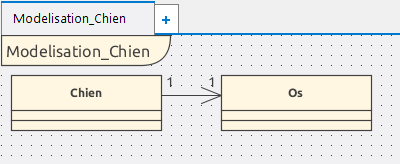
\includegraphics[width=0.95\linewidth]{images/partie_centrale.png}
		\caption{Diagramme de classes}
		\label{img:partie_centrale}
	\end{minipage}
\end{figure}

\section{Liste des éléments}
La partie de gauche de Slyum est une représentation sous forme d'arbre de tous les éléments UML existants dans le projet actuellement ouvert.

Les éléments sont classés dans cinq catégories représentées chacune par un noeud principal de l'arbre. Ces catégories sont Views (\ref{sec:vues}), Entities (\ref{sec:entites}), Relations (\ref{sec:relations}), Inheritances (\ref{sec:relations}), Dependencies (\ref{sec:relations}).

element en rouge

glisser déplacer

menu contextuel

sélection


\section{Propriétés des éléments}
